\section{Deep Learning and Neural Network}
\label{model:mlp}

\subsection{Overview}
As a subfield of machine learning, deep learning is formed as complex neural network architectures, containing more processing layers to learn hidden representations of the input data. This improvement is constructive in perceptual problems, where hand-crafted filters are merely impossible to achieve good results. In the following sections, we discuss from the original neural network to the further advanced ones.

\subsection{Perceptron}

\begin{figure}[!h]
    \centering
    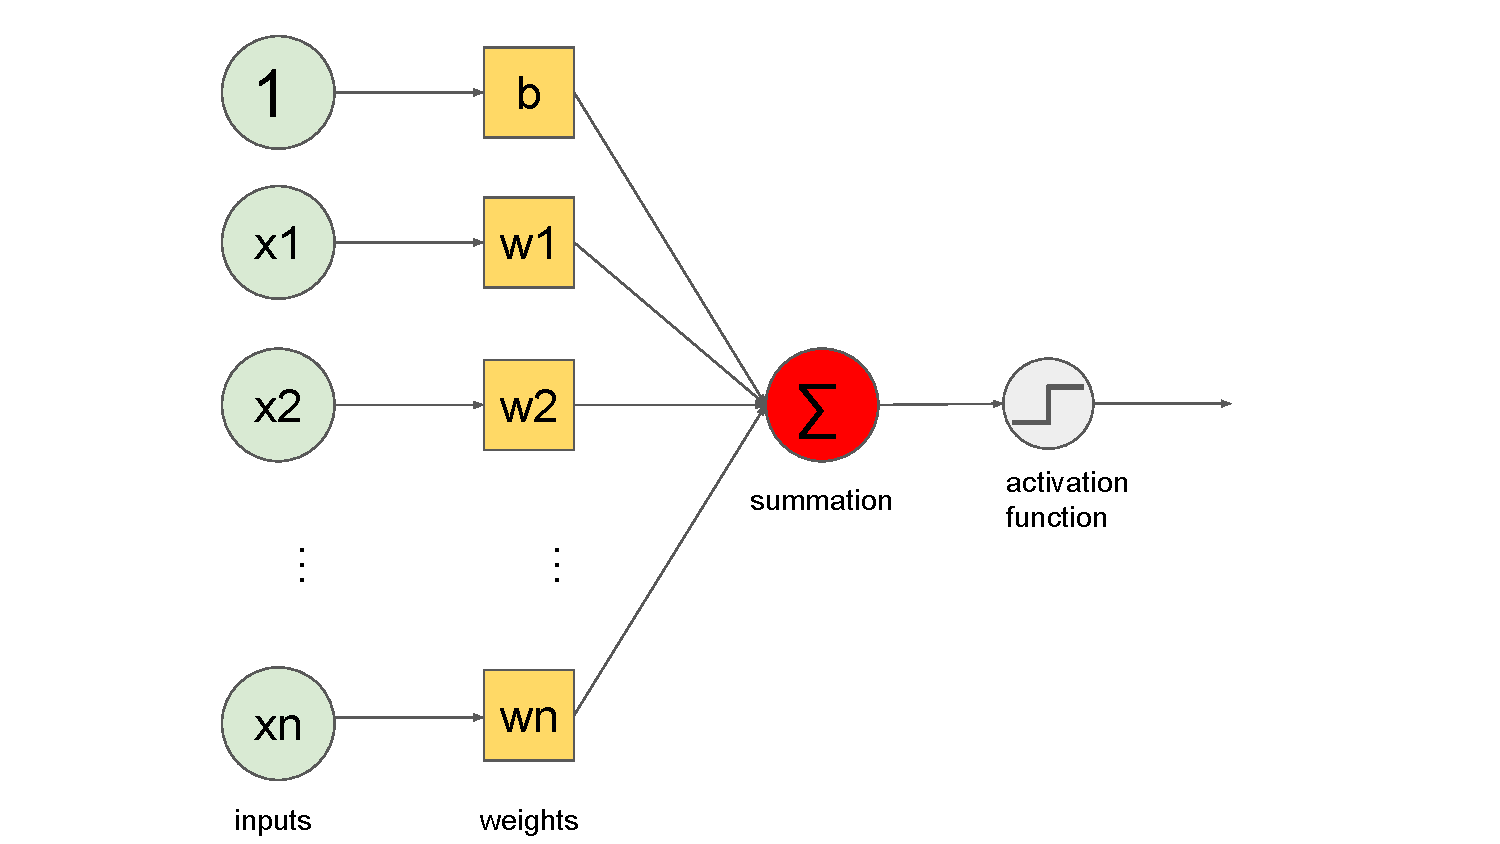
\includegraphics[width=\textwidth]{content/resources/new_images/related_works/perceptron.pdf}
    \caption{A single perceptron}
    \label{fig:perceptron}
\end{figure}

We first recap the early neural network, perceptron, which was introduced by Frank Rosenblatt in the 1950s \cite{rosenblatt1958perceptron} and 1960s \cite{rosenblatt1961principles}. 
The perceptron is an algorithm or a function for learning a binary classifier.
The function takes a $d$-dimensional vector $\mathbf{x}$ as input along with a weight vector $\mathbf{w}$ and calculates a single output value. 
\begin{align} \label{eqn: perceptron}
    a = f(\mathbf{x}) = \sigma(\mathbf{w}^T\mathbf{x} + b)
\end{align}
where $\mathbf{w}^T\mathbf{x} = \sum_{i=0}^{d} \omega_{i}x_{i} $ denotes the inner product between the input and weight vector and $b$ is bias. The perceptron behaves as a nonlinear function $\sigma$ of a linear combination of the input where each element $x_{i}$ is multiplied with it's corresponding coefficient $\omega_{i}$. 
Figure \ref{fig:perceptron} illustrates the process of a single perceptron process.\\
At first, the perceptron function is designed to solve the \textit{binary classification} problem in which each datapoint $\mathbf{x}$ belongs to a single class (denoted as \textbf{1} or \textbf{0}) and the weight vector $\mathbf{w}$ represents a boundary hyperplane that splits the space into two classes seperately. 
Therefore, points that lie at the same side of the plane are grouped to the same class. 
And the $sign$ function is used as activation function $\sigma$ in \ref{eqn: perceptron} to return $1$ if the combination is positive and $0$ otherwise.
\begin{align} \label{eqn: sgn_perceptron}
    a = f(\mathbf{x}) = \left\{\begin{matrix}
1 & \text{\quad if \quad} \mathbf{w}^T\mathbf{x} + b\geq 0 \\ 
0 & \text{\quad if \quad} \mathbf{w}^T\mathbf{x} + b <  0 
\end{matrix}\right.
\end{align}

\subsection{Activation functions}

Different from perceptron, activation function here is continuous, which makes the network weights differentiable with respect to output signals. \\
\begin{figure}[h]
    \centering
    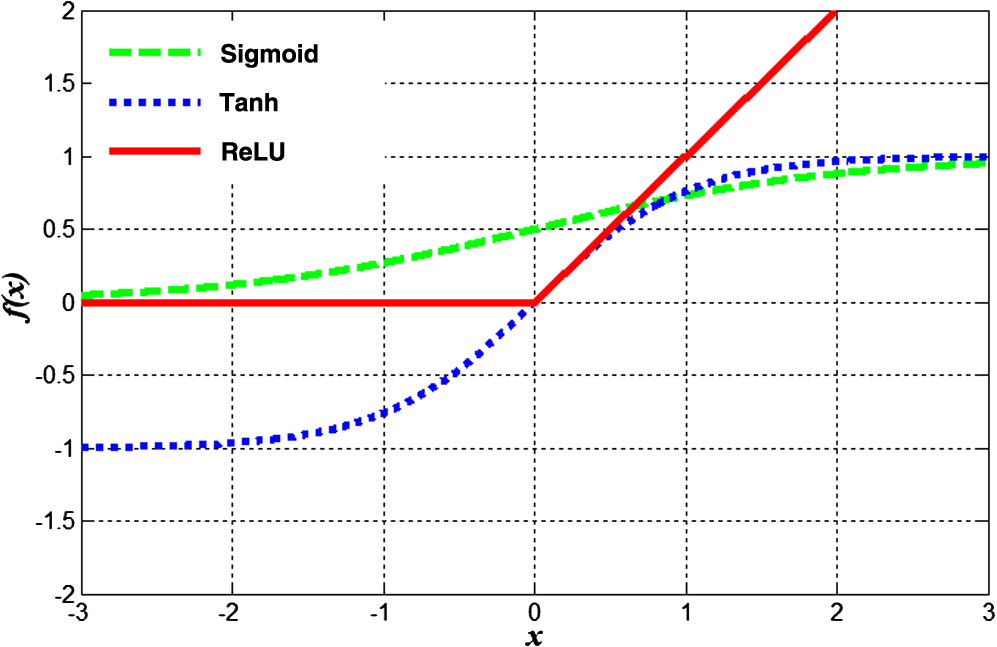
\includegraphics[width=0.7\textwidth]{resources/images/activation.png}
    \caption{Plot of Sigmoid, Tanh and ReLU activation functions.}
    \label{fig:activation}
\end{figure}
Here we list some of those activation functions commonly used in neural network modeling:
\begin{align} \label{eqn:sigmoid}
    \mathrm{sigmoid}(x) = \frac{1}{1 + \exp(-x)}
\end{align}
\begin{align} \label{eqn:tanh}
    \mathrm{tanh}(x) = \frac{\exp(2x - 1)}{\exp(2x + 1)} = 2 \times \mathrm{sigmoid}(2x) - 1
\end{align}
\begin{align} \label{eqn:relu}
    \mathrm{relu}(x) = \mathrm{max}(0, x)
\end{align}
The $sigmoid$ function (\ref{eqn:sigmoid}) scales real numbers to the range $[0, 1]$, where the large positive numbers change to $1$ and the large negative ones become $0$. Similar to $sigmoid$ but aims to produce zero-centered signals, $tanh$ function (\ref{eqn:tanh}) is a scaled version of $sigmoid$ with values range of $[-1, 1]$.\\
The drawback of both $sigmoid$ and $tanh$ is that when the numbers are large, the squashed values are saturated, hence their gradients is extremely small, which leads to the vanish problem when training deep neural networks. In such cases, Rectified Linear Unit ($ReLU$, \ref{eqn:relu}) is preferably used, which converts negative values to zero while keep the positive ones.
Figure \ref{fig:activation} illustrates the three functions in the same input range.



\subsection{Artificial Neural Networks}

The study of artificial neural networks (ANNs) has been inspired by the observation that biological learning systems are built of very complex webs of interconnected neurons in brains. The human brain contains a densely interconnected network of approximately trillion of neurons. ANN systems are motivated to capture this kind of highly parallel computation based on distributed representations. 

Generally, ANNs is a combination of a large number of interconnected processing neuron organized in a multi-layer architecture, where signal from a neuron can be passed to another from nearby layers (figure \ref{fig:neural_nets}). Each neuron is also formulated the same form as \ref{eqn: perceptron}. In general, neural network has an input layer, an output layer and a predefined number of hidden layers. Each hidden layer stands for a single transformation step in the process, which aims to extract hidden patterns of the input stored in it's neurons.  In recent years, state-of-the-art neural networks have multiple hidden layers. The number of layers determines the depth of the network, in contrast to the width of the network, which is determined by the maximum number of neurons between the hidden layers. In many cases, increasing depth increases the complexity of
the model, creates more space to store information and therefore increase its learning capability. These information is continually passed to following layers to extract more essential features. Due to the fact that sequence of linear transformations always equals to a single linear one, neural network uses nonlinear activation function $\sigma$ to element-wise apply to each processed neuron. 

\begin{figure}[h]
    \centering
    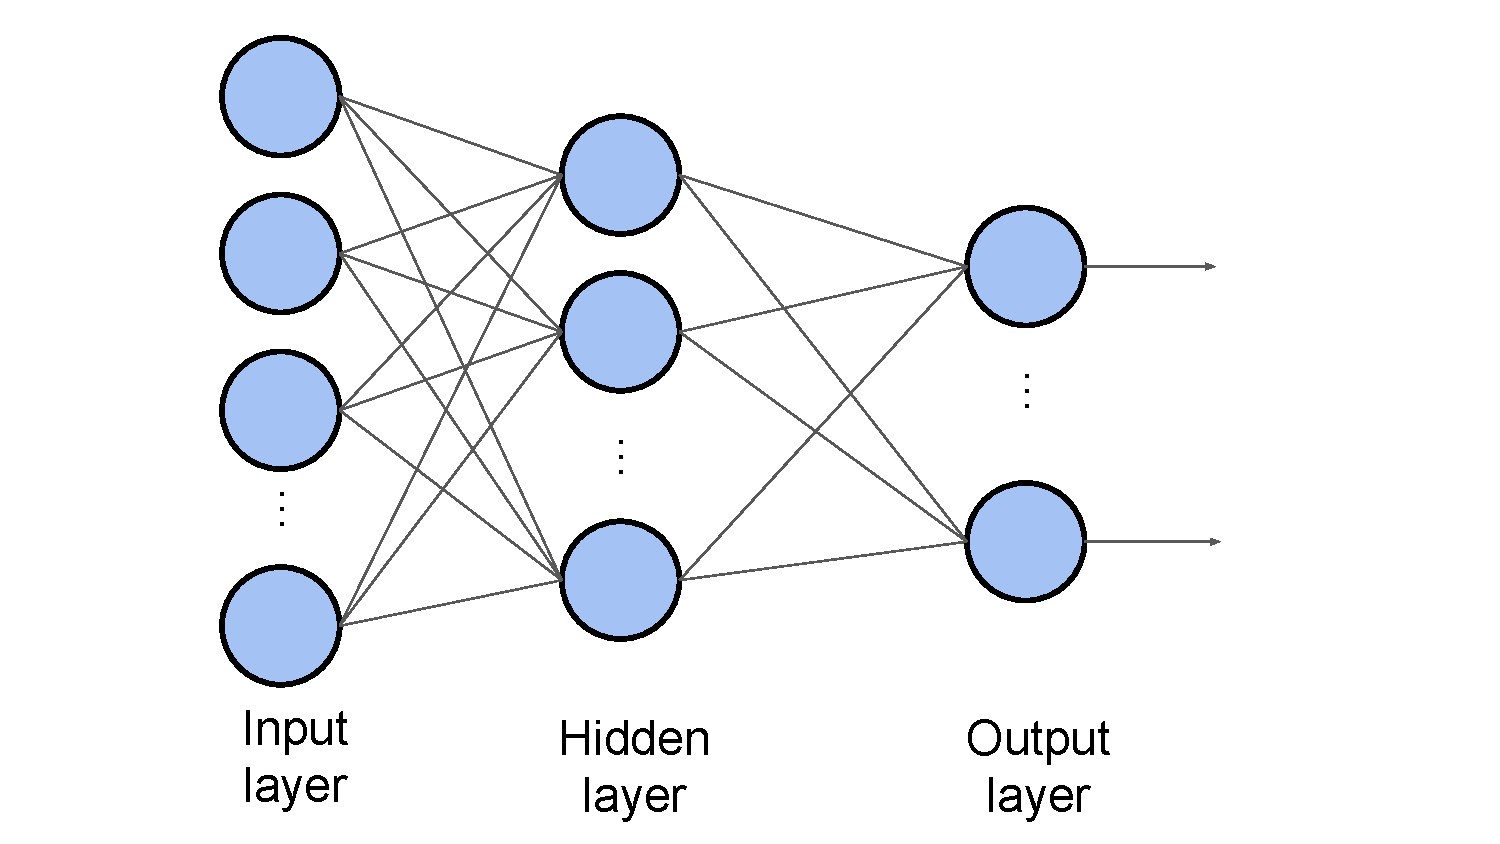
\includegraphics[width=0.7\textwidth]{content/resources/new_images/related_works/neural_nets.pdf}
    \caption{A simple three-layer neural network}
    \label{fig:neural_nets}
\end{figure}


Researchers have been actively conducting research on designing the architecture for ANNs to tackle machine learning and deep learning problem. Each new network design establishes on top of the older ones and each aims to solve a specific task independently. In order for the networks to deal with different tasks, such as classification, object detection, human action recognition, it cannot be without the usage of loss functions.

\subsection{Loss functions}

As stated in \ref{sec:ml}, supervised-learning neural networks must be trained with plenty of inputs-outputs data pairs. With every input, the network is expected to give a predictive outcome. While training, the network continuously adjusts its weights to minimize the discrepancy between its predicted outcome and the real outcome. The value of the discrepancy is often measured by using loss functions.

Loss functions are very diverse, each aims to solve different things and also is used for different tasks. For instance, in the regression task, the most used loss function is the least mean squared error. Suppose we have a model with parameters $\theta$, given a training sample $(x,y)$ where $x$ is the input and $y$ is the ground-truth, the loss for this single sample is calculated as follows

\begin{equation}
    \mathcal{L}(\theta,x,y) = \frac{1}{2} [y - h_{\theta}(x)]^2
\end{equation}

Similarly with classification task, the most frequently used one is cross-entropy loss. With the same notation as the example above, the loss function is as follows

\begin{equation}
    \mathcal{L}(\theta,x,y) = - (1-y_i) \text{log}(1-h_\theta(x_i)) - y_i\text{log}h_\theta(x_i)
\end{equation}

There are various factors involved in choosing a loss function for specific problem such as type of machine learning algorithm chosen, ease of calculating the derivatives and to some degree the percentage of outliers in the data set. 

So far, loss functions are used to determine the error between the output of our algorithms and the given target value. For the networks to perform better, it is essential to minimize the loss value. For only one training sample to be minimized, it is undoubtedly easy.
However, in practice, the loss value should be estimated for every possible training samples; this is nearly impossible. Therefore, the process of training can be formulated as an optimization problem: 

\begin{align}
    \mathcal{J}(\theta) &= E_{x,y} [L(\theta, x, y)] \approx \frac{1}{n} \sum^n_{i=1} L(\theta, x_i, y_i)
\end{align}

where $(x_i, y_i)$ is the $i^{th}$ oair and $n$ is the number of pairs in the dataset.
The target is to search for a set of parameters $\theta$ which minimize the expected loss function, or more realistically, calculate its approximation. An effective algorithm for this task is gradient descent, which is a fundamental tool of modern machine learning problems.

\subsection{Gradient descent}

Gradient descent (GD) is an iterative optimization algorithm used to find the local minimum of an objective function $J(\theta)$ by updating the parameters $\theta$ in the opposite direction of the gradient of that objective function. A gradient simply measures the change in all weights with regard to the change in error. In mathematical terms, a gradient is a partial derivative with respect to its inputs. 

How big the steps the GD takes into the direction of the local minimum are determined by the learning rate $\alpha$, which figures out how fast or slow we will move towards the optimal weights (as illustrated in Figure \ref{fig:gradient_descent}). Small value of $\alpha$ might lead to consistency but slow progress while larger one can result in faster progress but risk divergence. Thus, it must be carefully chosen. 

\begin{figure}[h]
    \centering
    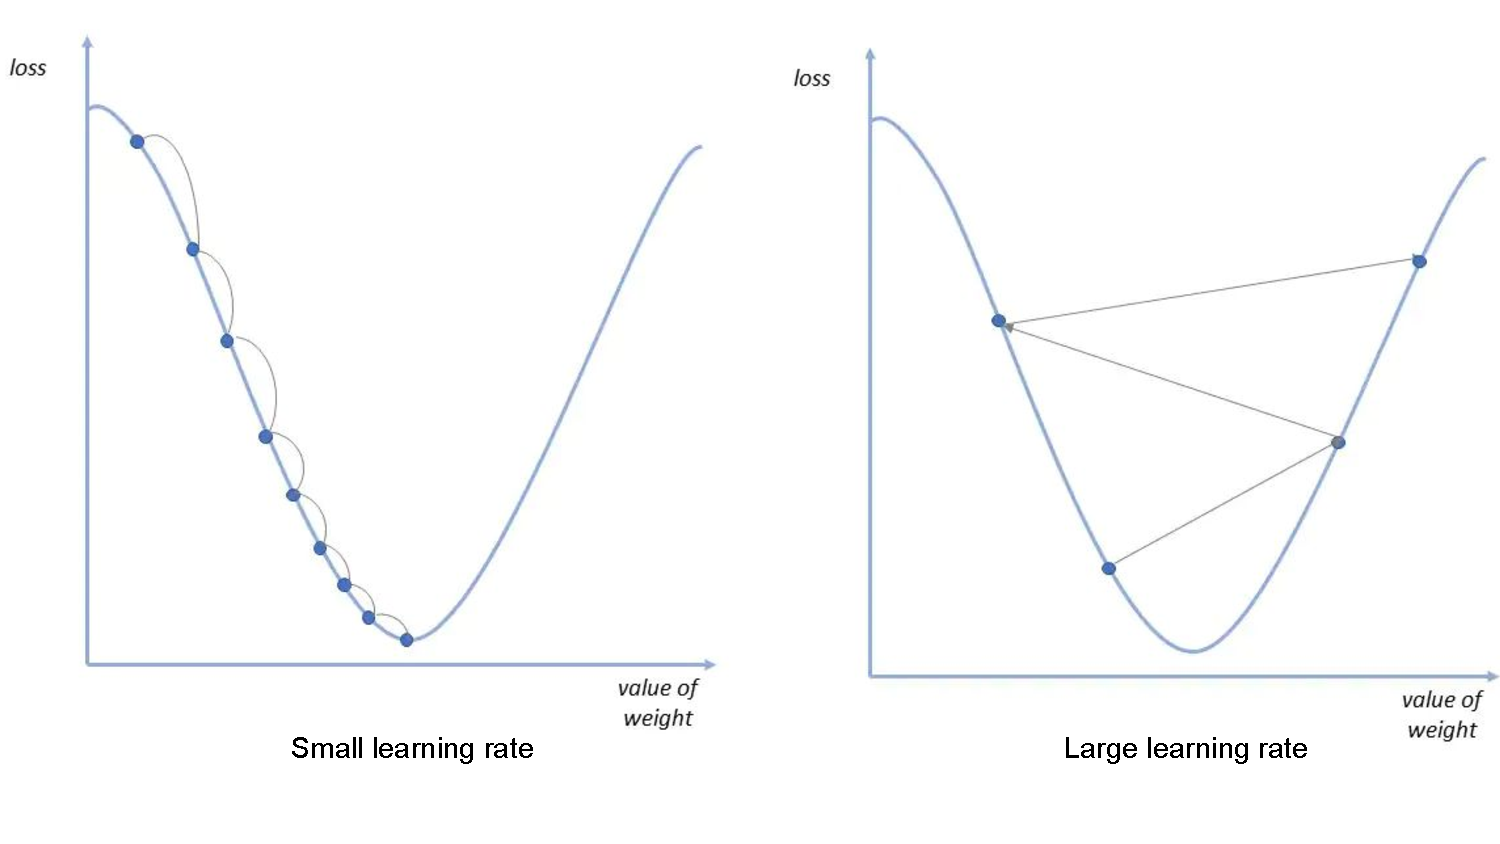
\includegraphics[width=0.9\textwidth]{content/resources/new_images/related_works/gradient_descent.pdf}
    \caption{Gradient descent}
    \label{fig:gradient_descent}
\end{figure}
 

Mathematically, the parameter $\theta_i$ in the set of parameters $\theta$ is updated as follows:

\begin{align}
    \theta_i := \theta_i - \alpha \frac{\partial J(\theta)}{\partial \theta_i}
\end{align}

While the original GD, also called vanilla GD, performs weights update after one pass through the whole dataset, which can be costly in practical scenario, there has been various variations that can alleviate this problem.
Stochastic gradient descent (SGD) \cite{bottou2010large} updates the parameters for each calculated training example one by one, which can help faster convergence than vanilla GD depending on the problem.  Additionally, the frequency of those updates can result in noisy gradients, which may cause the error rate to fluctuate instead of slowly decreasing. For the most strategic method, it must be the Mini-batch GD variant. It simply splits the training dataset into small batches and performs an update for each of those batches. From this variant, others with more parameters and mechanisms beside learning rate are introduced to improve the consistency and convergence speed of the algorithm, such as Adam \cite{kingma2014adam} or RMSProp.


\subsection{Feed-forward and Back-propagation}

\textbf{Feed-forward} describes the process of information flowing forward through the entire neural network. Given input data $x$, it is propagated through the intermediate layers to finally produce $\hat{y}$ at the output layer. Feed-forward is used both in the training and the testing phase to make predictions for any given input. In the training stage, the error is estimated between the network's output and ground truth; that essentially provides gradient information to update the network parameters. 

\textbf{Back-propagation} 
With the loss computed, back-propagation computes the gradient with respect to the weights of the network for a single input-output pair, and then flow the gradient information backward through the network . At each of the layers, new gradients are computed based on the following layers by the chain rule, then it is used to update the parameters in these layers using gradient descent. The process happens again until the gradients at the input layer are calculated and updated.

The process of feed-forward and back-propagation keep on repeating, and the weights keep updating continuously until the network becomes better fitted to the data that was fed into it, with reasonable evaluation result.
